% Options for packages loaded elsewhere
\PassOptionsToPackage{unicode}{hyperref}
\PassOptionsToPackage{hyphens}{url}
\PassOptionsToPackage{dvipsnames,svgnames,x11names}{xcolor}
%
\documentclass[
  letterpaper,
  DIV=11,
  numbers=noendperiod]{scrartcl}

\usepackage{amsmath,amssymb}
\usepackage{iftex}
\ifPDFTeX
  \usepackage[T1]{fontenc}
  \usepackage[utf8]{inputenc}
  \usepackage{textcomp} % provide euro and other symbols
\else % if luatex or xetex
  \usepackage{unicode-math}
  \defaultfontfeatures{Scale=MatchLowercase}
  \defaultfontfeatures[\rmfamily]{Ligatures=TeX,Scale=1}
\fi
\usepackage{lmodern}
\ifPDFTeX\else  
    % xetex/luatex font selection
\fi
% Use upquote if available, for straight quotes in verbatim environments
\IfFileExists{upquote.sty}{\usepackage{upquote}}{}
\IfFileExists{microtype.sty}{% use microtype if available
  \usepackage[]{microtype}
  \UseMicrotypeSet[protrusion]{basicmath} % disable protrusion for tt fonts
}{}
\makeatletter
\@ifundefined{KOMAClassName}{% if non-KOMA class
  \IfFileExists{parskip.sty}{%
    \usepackage{parskip}
  }{% else
    \setlength{\parindent}{0pt}
    \setlength{\parskip}{6pt plus 2pt minus 1pt}}
}{% if KOMA class
  \KOMAoptions{parskip=half}}
\makeatother
\usepackage{xcolor}
\setlength{\emergencystretch}{3em} % prevent overfull lines
\setcounter{secnumdepth}{5}
% Make \paragraph and \subparagraph free-standing
\makeatletter
\ifx\paragraph\undefined\else
  \let\oldparagraph\paragraph
  \renewcommand{\paragraph}{
    \@ifstar
      \xxxParagraphStar
      \xxxParagraphNoStar
  }
  \newcommand{\xxxParagraphStar}[1]{\oldparagraph*{#1}\mbox{}}
  \newcommand{\xxxParagraphNoStar}[1]{\oldparagraph{#1}\mbox{}}
\fi
\ifx\subparagraph\undefined\else
  \let\oldsubparagraph\subparagraph
  \renewcommand{\subparagraph}{
    \@ifstar
      \xxxSubParagraphStar
      \xxxSubParagraphNoStar
  }
  \newcommand{\xxxSubParagraphStar}[1]{\oldsubparagraph*{#1}\mbox{}}
  \newcommand{\xxxSubParagraphNoStar}[1]{\oldsubparagraph{#1}\mbox{}}
\fi
\makeatother


\providecommand{\tightlist}{%
  \setlength{\itemsep}{0pt}\setlength{\parskip}{0pt}}\usepackage{longtable,booktabs,array}
\usepackage{calc} % for calculating minipage widths
% Correct order of tables after \paragraph or \subparagraph
\usepackage{etoolbox}
\makeatletter
\patchcmd\longtable{\par}{\if@noskipsec\mbox{}\fi\par}{}{}
\makeatother
% Allow footnotes in longtable head/foot
\IfFileExists{footnotehyper.sty}{\usepackage{footnotehyper}}{\usepackage{footnote}}
\makesavenoteenv{longtable}
\usepackage{graphicx}
\makeatletter
\def\maxwidth{\ifdim\Gin@nat@width>\linewidth\linewidth\else\Gin@nat@width\fi}
\def\maxheight{\ifdim\Gin@nat@height>\textheight\textheight\else\Gin@nat@height\fi}
\makeatother
% Scale images if necessary, so that they will not overflow the page
% margins by default, and it is still possible to overwrite the defaults
% using explicit options in \includegraphics[width, height, ...]{}
\setkeys{Gin}{width=\maxwidth,height=\maxheight,keepaspectratio}
% Set default figure placement to htbp
\makeatletter
\def\fps@figure{htbp}
\makeatother
% definitions for citeproc citations
\NewDocumentCommand\citeproctext{}{}
\NewDocumentCommand\citeproc{mm}{%
  \begingroup\def\citeproctext{#2}\cite{#1}\endgroup}
\makeatletter
 % allow citations to break across lines
 \let\@cite@ofmt\@firstofone
 % avoid brackets around text for \cite:
 \def\@biblabel#1{}
 \def\@cite#1#2{{#1\if@tempswa , #2\fi}}
\makeatother
\newlength{\cslhangindent}
\setlength{\cslhangindent}{1.5em}
\newlength{\csllabelwidth}
\setlength{\csllabelwidth}{3em}
\newenvironment{CSLReferences}[2] % #1 hanging-indent, #2 entry-spacing
 {\begin{list}{}{%
  \setlength{\itemindent}{0pt}
  \setlength{\leftmargin}{0pt}
  \setlength{\parsep}{0pt}
  % turn on hanging indent if param 1 is 1
  \ifodd #1
   \setlength{\leftmargin}{\cslhangindent}
   \setlength{\itemindent}{-1\cslhangindent}
  \fi
  % set entry spacing
  \setlength{\itemsep}{#2\baselineskip}}}
 {\end{list}}
\usepackage{calc}
\newcommand{\CSLBlock}[1]{\hfill\break\parbox[t]{\linewidth}{\strut\ignorespaces#1\strut}}
\newcommand{\CSLLeftMargin}[1]{\parbox[t]{\csllabelwidth}{\strut#1\strut}}
\newcommand{\CSLRightInline}[1]{\parbox[t]{\linewidth - \csllabelwidth}{\strut#1\strut}}
\newcommand{\CSLIndent}[1]{\hspace{\cslhangindent}#1}

\usepackage{booktabs}
\usepackage{longtable}
\usepackage{array}
\usepackage{multirow}
\usepackage{wrapfig}
\usepackage{float}
\usepackage{colortbl}
\usepackage{pdflscape}
\usepackage{tabu}
\usepackage{threeparttable}
\usepackage{threeparttablex}
\usepackage[normalem]{ulem}
\usepackage{makecell}
\usepackage{xcolor}
\KOMAoption{captions}{tableheading}
\makeatletter
\@ifpackageloaded{caption}{}{\usepackage{caption}}
\AtBeginDocument{%
\ifdefined\contentsname
  \renewcommand*\contentsname{Table of contents}
\else
  \newcommand\contentsname{Table of contents}
\fi
\ifdefined\listfigurename
  \renewcommand*\listfigurename{List of Figures}
\else
  \newcommand\listfigurename{List of Figures}
\fi
\ifdefined\listtablename
  \renewcommand*\listtablename{List of Tables}
\else
  \newcommand\listtablename{List of Tables}
\fi
\ifdefined\figurename
  \renewcommand*\figurename{Figure}
\else
  \newcommand\figurename{Figure}
\fi
\ifdefined\tablename
  \renewcommand*\tablename{Table}
\else
  \newcommand\tablename{Table}
\fi
}
\@ifpackageloaded{float}{}{\usepackage{float}}
\floatstyle{ruled}
\@ifundefined{c@chapter}{\newfloat{codelisting}{h}{lop}}{\newfloat{codelisting}{h}{lop}[chapter]}
\floatname{codelisting}{Listing}
\newcommand*\listoflistings{\listof{codelisting}{List of Listings}}
\makeatother
\makeatletter
\makeatother
\makeatletter
\@ifpackageloaded{caption}{}{\usepackage{caption}}
\@ifpackageloaded{subcaption}{}{\usepackage{subcaption}}
\makeatother

\ifLuaTeX
  \usepackage{selnolig}  % disable illegal ligatures
\fi
\usepackage{bookmark}

\IfFileExists{xurl.sty}{\usepackage{xurl}}{} % add URL line breaks if available
\urlstyle{same} % disable monospaced font for URLs
\hypersetup{
  pdftitle={Forecasting the 2024 US Presidential Election},
  pdfauthor={Tina Kim; David Flores; Kevin Shao},
  colorlinks=true,
  linkcolor={blue},
  filecolor={Maroon},
  citecolor={Blue},
  urlcolor={Blue},
  pdfcreator={LaTeX via pandoc}}


\title{Forecasting the 2024 US Presidential Election\thanks{Code and
data are available at:
https://github.com/DavidFJ207/USPresidentialForecast}}
\usepackage{etoolbox}
\makeatletter
\providecommand{\subtitle}[1]{% add subtitle to \maketitle
  \apptocmd{\@title}{\par {\large #1 \par}}{}{}
}
\makeatother
\subtitle{Analyzing Demographic Patterns and Predicting Swing States}
\author{Tina Kim \and David Flores \and Kevin Shao}
\date{November 3, 2024}

\begin{document}
\maketitle
\begin{abstract}
Our analysis of swing state polls for the 2024 U.S. Presidential
Election shows a close race. Republicans lead in most key states like
Michigan, Georgia, Nevada, Wisconsin, and Pennsylvania, while Democrats
have a slight edge in Arizona. The national average also leans
Republican, suggesting a Republican win in the 2024 Election.
\end{abstract}


\section{Introduction}\label{introduction}

\emph{Overview paragraph:} The 2024 United States of America
Presidential Election is to elect the fourty-seventh president of USA,
with the two candidates as Donald Trump, the fourty-fifth president of
the United States and representative of the Republican Party, and Kamala
Harris, current vice president of the United States and representative
of the Democratic Party, after Joe Biden announced that he will not
continue participate in this presidential election anymore (Jr (2024)).
Democracy can be described as liberal and left-leaning, with the
emphasis of economy intervention with implementation of policies such as
minimum wage and progressive tax rates. Members of the Republican party
tend to follow the free economy, and can be described as right-leaning
({``Democrat Vs. Republican''} (n.d.)). The results of the 2024
Presidential Election will determine which political party, Republican
or Democratic, will become the leader of the United States for the next
four years, largely affecting the policies implemented in the United
States during this time period. Due to the strong nation power of the
United States, this may even affect the world's economic trends in the
four years. Therefore, predicting results of the upcoming 2024 United
States Presidential Election is a necessary action.

\emph{Estimand paragraph:} To predict results of the 2024 United States
of America Presidential Election, our aim is clearly to conclude which
candidate, either Harris or Trump, is more likely to win this election.
Our response variable is in turn the probability of one candidate
winning the election based on poll data, with our chosen poll as
Emerson. When the supporting percentage of one candidate, or the party
s/he represents, is only slightly less than 50\%, we cannot clearly
determine whether s/he would be predicted to have been elected as the
fourty-seventh US President or not, since there is a group of people who
did not choose to participate in the voting process. Therefore, to
increase accuracy of predictions, we will build two models, one model
with the estimand as the probability of Harris, or the Democratic party,
winning the election, and another with the estimand as the probability
of Trump, or the Republican party, winning the election. By comparing
the two predictions, one can get a final prediction of who is more
likely to be elected as the next President of the United States of
America.

\emph{Results paragraph:} Summarize the key findings of the model,
highlighting its predictive accuracy and implications.

\emph{Why it matters paragraph:} Explain the broader significance of
accurately forecasting election results for politics, society, and
policymaking.

\emph{Telegraphing paragraph:} The remainder of this paper is structured
as follows: Section 2 details the data and measurement process; Section
3 covers model development and results; Section 4 discusses implications
and future steps. The remainder of this paper is structured as follows.
Section~\ref{sec-data}\ldots.

\section{Data}\label{sec-data}

\subsection{Overview}\label{overview}

We sourced the ``Presidential General Election Polls'' dataset from
FiveThirtyEight (FiveThirtyEight 2024) and performed an in-depth
analysis using the statistical programming language R (R Core Team
2023).

Our primary objective was to clean, organize, and analyze U.S.
presidential election polling data to provide insights into voter
preferences by state. This involved selecting data from reputable
pollsters, organizing it by state, and addressing any missing or
incomplete entries. Additional datasets were merged where necessary, and
after thoroughly addressing missing values, we finalized a polished
dataset ready for analysis. Below is a table summarizing the polling
data by state, showcasing voter preferences by party and demographic
breakdowns. The table highlights key trends and differences across
states in terms of party lean and demographic distribution.
Figure~\ref{fig-predictors-pct-summary-1} and
Figure~\ref{fig-predictors-pct-summary-2} provides a snapshot of these
findings.

\begin{figure}

\centering{

\begingroup\fontsize{10}{12}\selectfont

\begin{longtable*}[t]{lrrrr}
\toprule
State & Democrat Pct & Republican Pct & Voted Biden 2020 & Voted Trump 2020\\
\midrule
Arizona & 48.2 & 50.5 & 46.0 & 45.2\\
Georgia & 49.8 & 49.7 & 44.5 & 44.3\\
Michigan & 49.7 & 49.6 & 57.9 & 26.8\\
Nevada & 49.2 & 48.1 & 57.9 & 26.8\\
New Hampshire & 50.9 & 47.2 & 51.8 & 35.8\\
\addlinespace
North Carolina & 48.2 & 50.2 & 46.0 & 45.2\\
Pennsylvania & 49.0 & 50.7 & 45.3 & 44.9\\
Wisconsin & 49.2 & 49.9 & 58.2 & 28.7\\
\bottomrule
\end{longtable*}
\endgroup{}

}

\caption{\label{fig-predictors-pct-summary-1}}

\end{figure}%

\begin{figure}

\centering{

\begingroup\fontsize{6}{8}\selectfont

\begin{longtable*}[t]{lrrrrrrr}
\toprule
State & High Educated & Low Educated & Female & Male & Nonbinary & Caucasian & Minority Ethnicity\\
\midrule
Arizona & 22.1 & 24.3 & 51.8 & 46.4 & 1.8 & 80.2 & 19.8\\
Georgia & 23.8 & 24.1 & 49.8 & 49.5 & 0.7 & 86.5 & 13.5\\
Michigan & 27.2 & 22.6 & 53.0 & 46.2 & 0.8 & 60.3 & 39.7\\
Nevada & 27.2 & 22.6 & 53.0 & 46.2 & 0.8 & 60.3 & 39.7\\
New Hampshire & 30.1 & 17.7 & 52.5 & 46.7 & 0.8 & 68.3 & 31.7\\
\addlinespace
North Carolina & 22.1 & 24.3 & 51.8 & 46.4 & 1.8 & 80.2 & 19.8\\
Pennsylvania & 25.8 & 21.8 & 53.7 & 44.6 & 1.7 & 60.9 & 39.1\\
Wisconsin & 28.7 & 19.5 & 51.9 & 47.1 & 1.0 & 49.1 & 50.9\\
\bottomrule
\end{longtable*}
\endgroup{}

}

\caption{\label{fig-predictors-pct-summary-2}}

\end{figure}%

Latest Poll Points by Party

\subsection{Measurement}\label{measurement}

We chose Emerson as our primary pollster, and the reasoning for this is
detailed in \textbf{?@sec-appenA}. Emerson's polls offered crucial
information, such as polling dates, party affiliations, sample sizes,
and the percentage of support for each political party.

Our analysis centered on voter preferences by party rather than
individual candidates. This approach was more relevant for identifying
overall trends and helped us forecast which states might swing in future
elections, especially swing states. We will discuss this focus further
in our results section, Section~\ref{sec-results}.

The Emerson dataset also included valuable demographic data, voting
history, and approval ratings. To ensure a consistent analysis, we
concentrated on questions that were uniformly asked across all states.
This approach allowed us to aggregate and analyze data at the state
level without being limited by state-specific polling variations.

\subsection{Outcome Variables}\label{outcome-variables}

Our initial analysis of the dataset revealed important trends in party
preferences across states. In Figure~\ref{fig-party-results}, we show
which states have the strongest leanings toward the Democratic or
Republican parties. This visualization is crucial for identifying key
swing states, which lie near the center of the graph and show nearly
equal support for both parties. These states are especially important
for predicting the 2024 election outcome.

From this analysis, we identified eight critical swing states: Michigan,
Georgia, Nevada, North Carolina, New Hampshire, Wisconsin, Pennsylvania,
and Arizona. These states will be central to our election prediction.
Although Minnesota emerged as a potential swing state, we excluded it
due to the wide range of polling data, as explained in
Table~\ref{tbl-final-summary}. Additionally, we will consider the
national average in our overall prediction.

\begin{figure}

\centering{

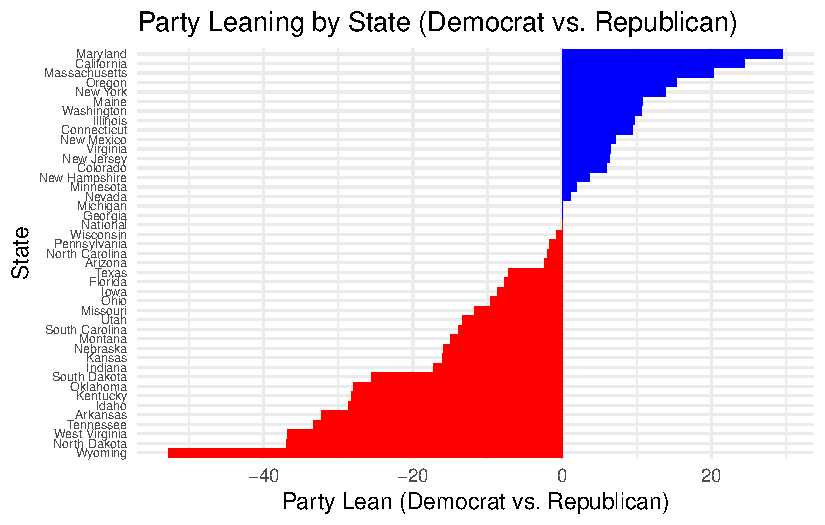
\includegraphics{paper_files/figure-pdf/fig-party-results-1.pdf}

}

\caption{\label{fig-party-results}Example Predictor Variable
Visualization}

\end{figure}%

\begin{longtable}[]{@{}
  >{\raggedright\arraybackslash}p{(\columnwidth - 12\tabcolsep) * \real{0.1546}}
  >{\raggedleft\arraybackslash}p{(\columnwidth - 12\tabcolsep) * \real{0.1340}}
  >{\raggedleft\arraybackslash}p{(\columnwidth - 12\tabcolsep) * \real{0.1443}}
  >{\raggedleft\arraybackslash}p{(\columnwidth - 12\tabcolsep) * \real{0.1443}}
  >{\raggedleft\arraybackslash}p{(\columnwidth - 12\tabcolsep) * \real{0.1340}}
  >{\raggedleft\arraybackslash}p{(\columnwidth - 12\tabcolsep) * \real{0.1443}}
  >{\raggedleft\arraybackslash}p{(\columnwidth - 12\tabcolsep) * \real{0.1443}}@{}}

\caption{\label{tbl-final-summary}Final Summary Table of 95\% Confidence
Intervals for Common States}

\tabularnewline

\toprule\noalign{}
\begin{minipage}[b]{\linewidth}\raggedright
State
\end{minipage} & \begin{minipage}[b]{\linewidth}\raggedleft
DEM Mean (\%)
\end{minipage} & \begin{minipage}[b]{\linewidth}\raggedleft
DEM Lower 95\%
\end{minipage} & \begin{minipage}[b]{\linewidth}\raggedleft
DEM Upper 95\%
\end{minipage} & \begin{minipage}[b]{\linewidth}\raggedleft
REP Mean (\%)
\end{minipage} & \begin{minipage}[b]{\linewidth}\raggedleft
REP Lower 95\%
\end{minipage} & \begin{minipage}[b]{\linewidth}\raggedleft
REP Upper 95\%
\end{minipage} \\
\midrule\noalign{}
\endhead
\bottomrule\noalign{}
\endlastfoot
Arizona & 42.5 & 40.8 & 44.2 & 47.1 & 45.7 & 48.5 \\
Georgia & 42.8 & 41.0 & 44.7 & 47.8 & 46.7 & 48.9 \\
Michigan & 44.9 & 43.4 & 46.4 & 45.6 & 44.3 & 46.9 \\
National & 42.4 & 41.5 & 43.3 & 43.7 & 42.5 & 44.9 \\
Nevada & 41.8 & 39.6 & 44.0 & 45.9 & 44.6 & 47.2 \\
New Hampshire & 44.8 & 42.6 & 47.0 & 41.6 & 39.9 & 43.4 \\
North Carolina & 43.2 & 40.4 & 46.0 & 48.6 & 47.7 & 49.6 \\
Pennsylvania & 44.2 & 42.5 & 45.9 & 47.6 & 46.6 & 48.6 \\
Wisconsin & 44.4 & 42.7 & 46.0 & 46.5 & 45.2 & 47.8 \\

\end{longtable}

\begin{figure}

\centering{

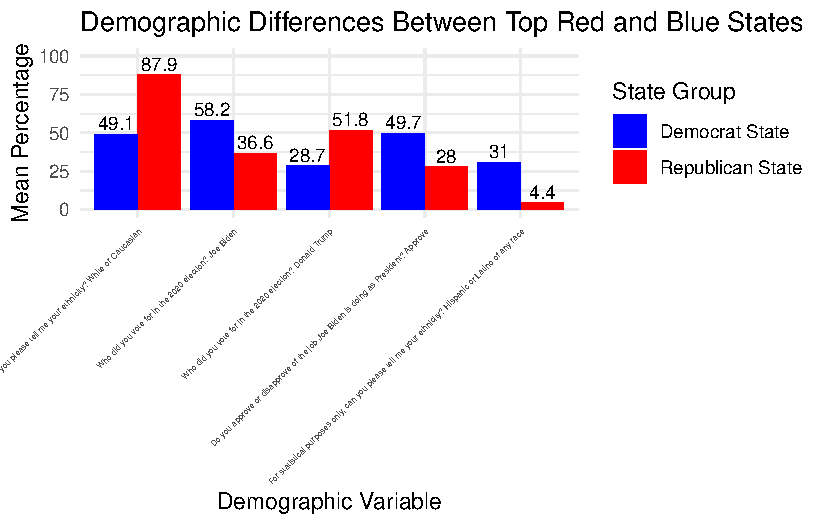
\includegraphics{paper_files/figure-pdf/fig-party-extremes-1.pdf}

}

\caption{\label{fig-party-extremes}Demographic Differences Between Top
Red and Blue States}

\end{figure}%

Beyond identifying swing states, it's also important to understand the
differences between the strongest Democratic (``blue'') and Republican
(``red'') states. The bar graph in Figure~\ref{fig-party-extremes}
highlights these differences. It focuses on key factors that create the
biggest contrasts between Democratic-leaning and Republican-leaning
states, helping to show how these factors differ between the most
extreme red and blue states.

To start, the graph features two bars, one for Democratic points and one
for Republican points, reflecting the responses to questions asked by
Emerson Pollster about voting intentions. These responses closely align
with the percentages shown for each state, giving us a clear picture of
voter preferences.

The Figure~\ref{fig-party-extremes} visualization gives us valuable
insight into how people's poll responses may influence their political
leanings.

Through these visualizations, we not only identify which states are most
likely to swing in future elections but also better understand the
public opinions driving these partisan divides.

\subsection{Predictor Variables}\label{predictor-variables}

We then take a closer look at the demographic and social factors that
shape voter preferences. The predictors we analyze include education
levels, gender, and past voting behavior. These variables are important
because they significantly impact political leanings and can influence
how a state is likely to vote.

In Figure~\ref{fig-predictors-party-pct}, we examine how these factors
correlate with party lean across U.S. states. This analysis helps
identify which factors have the greatest influence in each state,
providing a clearer understanding of what drives voter behavior.

\begin{figure}

\centering{

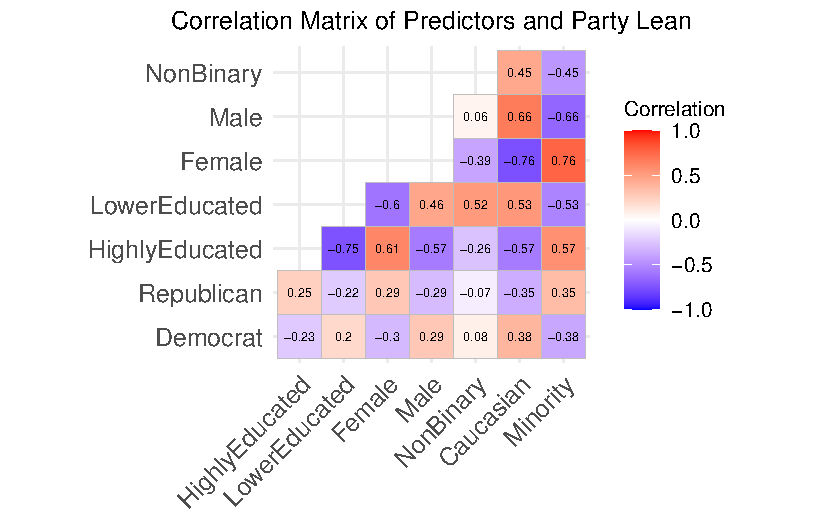
\includegraphics{paper_files/figure-pdf/fig-predictors-party-pct-1.pdf}

}

\caption{\label{fig-predictors-party-pct}Example Predictor Variable
Visualization}

\end{figure}%

\begin{figure}

\centering{

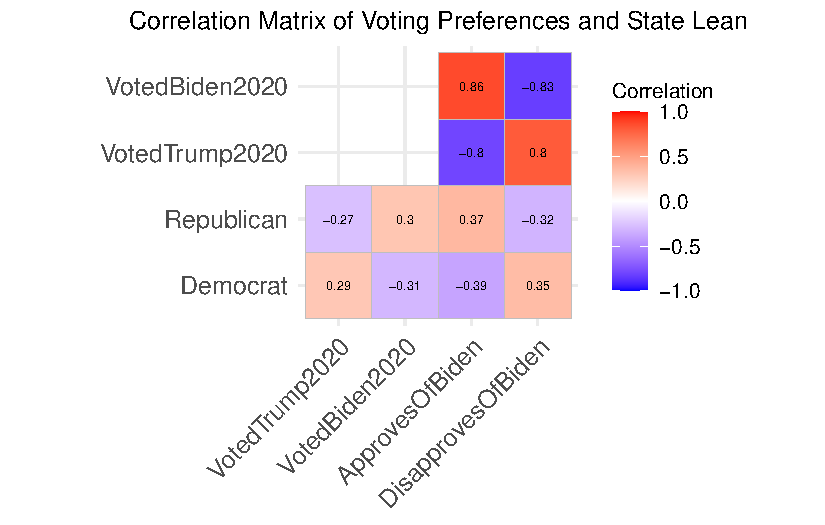
\includegraphics{paper_files/figure-pdf/fig-predictors-party-pct-2-1.pdf}

}

\caption{\label{fig-predictors-party-pct-2}Example Voting and Approval
Predictor Variable Visualization}

\end{figure}%

\begin{figure}

\centering{

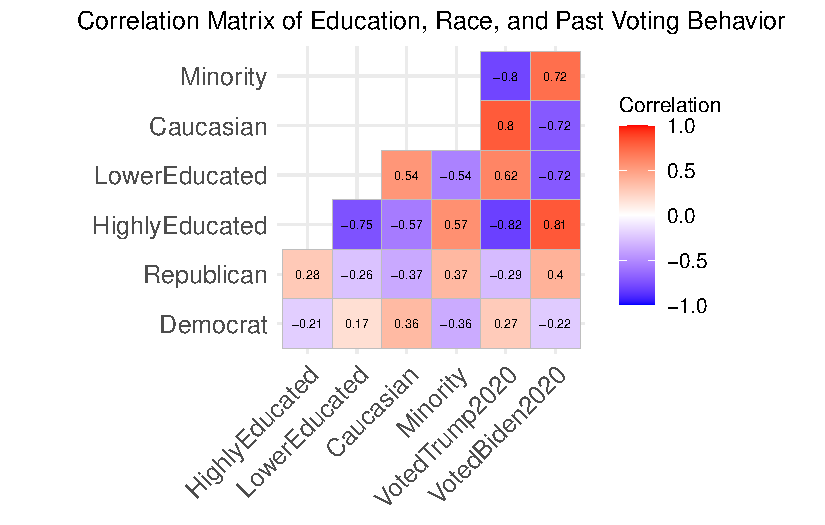
\includegraphics{paper_files/figure-pdf/fig-predictors-education-race-voting-1.pdf}

}

\caption{\label{fig-predictors-education-race-voting}Correlation Matrix
of Education, Race, and Past Voting Behavior}

\end{figure}%

The correlation matrix in Figure~\ref{fig-predictors-party-pct} shows
how different predictors relate to party preferences. We can see which
factors, like education or gender, are more strongly tied to Democratic
or Republican leanings. Blue shading indicates stronger Democratic
support, while red shows stronger Republican support. Key observations
include higher education being linked to Democratic support and lower
education favoring Trump in 2020. Minority groups generally lean
Democratic, while Caucasian/White voters tend to support Trump. Past
voter behavior shows Biden supporters remain Democratic, and Trump
supporters disapprove of Biden. Additionally, women lean slightly more
Democratic compared to men, who often lean Republican.

\begin{figure}

\centering{

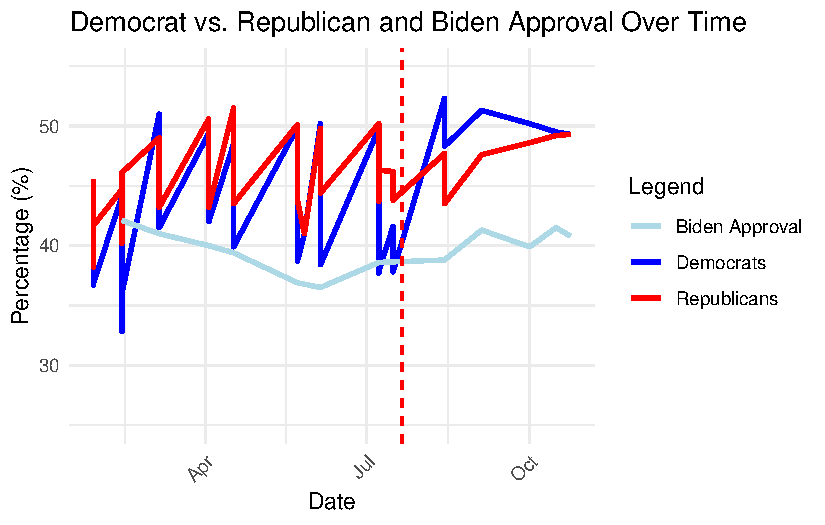
\includegraphics{paper_files/figure-pdf/fig-points-over-time-1.pdf}

}

\caption{\label{fig-points-over-time}}

\end{figure}%

Lastly, we examine Democratic and Republican support alongside Biden's
approval over time, marking July 21st when Joe Biden concluded his
campaign, as reported by Rabson (2024). During this period, Democratic
support was initially low but increased following this change. By
analyzing specific demographic factors and previous voting behavior, we
aim to predict the 2024 election outcome.

Key predictor variables:

\begin{itemize}
\tightlist
\item
  \textbf{Education}: This measures education levels, with higher
  education often correlating with more Democratic support.
\item
  \textbf{Race/Ethnicity}: This examines how different racial and ethnic
  groups tend to align politically, with minority groups often leaning
  Democratic and White/Caucasian voters leaning Republican.
\item
  \textbf{Gender}: This captures how gender influences party preference,
  with women generally leaning more Democratic and men more Republican.
\item
  \textbf{Priors (Past Voting Behavior)}: This looks at who people voted
  for in the past, helping us understand ongoing political support or
  disapproval.
\item
  \textbf{Biden's Approval Rating}: This assesses how approval or
  disapproval of Joe Biden impacts Democratic support, providing insight
  into shifting voter sentiments.
\end{itemize}

\section{Model}\label{sec-model}

\subsection{Model Development}\label{model-development}

The goal of our model is to forecast the popular vote outcome of the
2024 US presidential election, focusing specifically on eight swing
states. We will choose the predictor variables based on the correlation
matrix we created previously (Figure~\ref{fig-predictors-party-pct}). It
is important to note that even if the percentage of people who vote for
Trump (representing the Republican Party) or Harris (representing the
Democratic Party) is slightly below 50\%, this does not necessarily mean
that the corresponding candidate will not be elected as the next
President of the United States, given the percentage of people who
choose not to vote.

\begin{figure}

\centering{

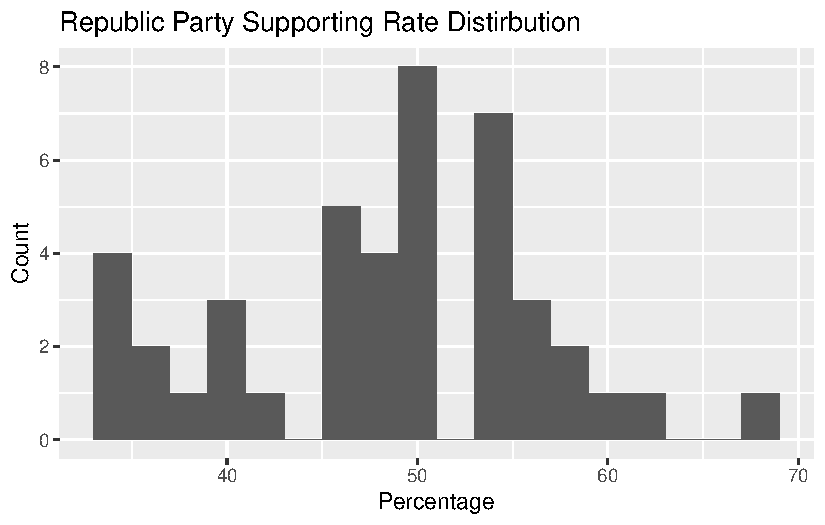
\includegraphics{paper_files/figure-pdf/fig-hist-for-republican-1.pdf}

}

\caption{\label{fig-hist-for-republican}Distribution of Republican Party
Supporting Rate}

\end{figure}%

The following Figure~\ref{fig-hist-for-democratic} is the histogram of
the Democratic Party Supporting Rate, which describes the distribution
of the response variable for the second model. Our final choice is to
construct two generalized linear models: one for the percentage that
Trump will become the next President and one for Harris. We can then
compare the predicted percentages of people voting for each candidate to
make a final prediction of who is more likely to be the next President
of the United States.

\begin{figure}

\centering{

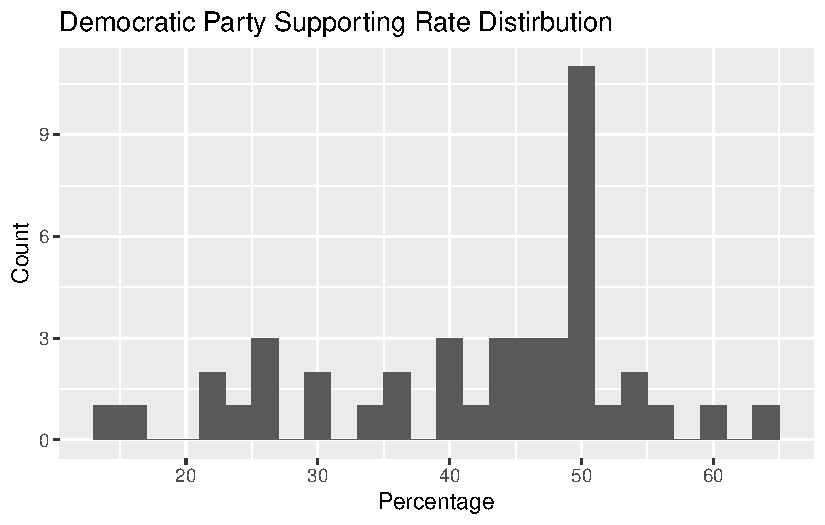
\includegraphics{paper_files/figure-pdf/fig-hist-for-democratic-1.pdf}

}

\caption{\label{fig-hist-for-democratic}Distribution of Democratic Party
Supporting Rate}

\end{figure}%

To decide between using a generalized linear model or a linear model for
each of the two models, we checked the normality of the response
variables: the percentage of people supporting the Republican Party and
the percentage supporting the Democratic Party. According to
Figure~\ref{fig-hist-for-democratic} and
Figure~\ref{fig-hist-for-republican}, the distributions of both response
variables do not appear normal. The distribution of the Democratic Party
Supporting Rate tends to resemble a Poisson distribution, with most
percentages having a similar frequency and an outlier around 67-68
percent. The Republican Party Supporting Rate distribution has a maximum
frequency around 50 percent, with similar frequencies around 25-26
percent and 48-49 percent, suggesting a potential violation of the
normal distribution assumption.

Therefore, since the response variables are not normally distributed, we
will use a generalized linear model for both models to better capture
the characteristics of the data.

The goal of our model is to forecast the likely vote outcome in 8 swing
states for the 2024 US presidential election. This model will allow us
to estimate the expected vote share for each candidate based on
state-level characteristics and prior voting patterns, which are
especially important in determining close elections.

\subsection{Model Set-up}\label{model-set-up}

We define the model as a Bayesian linear model where the outcome, ( y\_i
), represents the predicted vote share in state ( i ). The predictors in
the model capture key demographic and historical voting patterns across
swing states, and we aim to model this outcome with an intercept, (
\alpha ), and a state-specific predictor coefficient, ( \beta\_i ), that
represents the effect of a given variable ( x\_i ) on vote share.

\subsubsection{Model Components and
Assumptions}\label{model-components-and-assumptions}

\begin{itemize}
\tightlist
\item
  \textbf{Outcome Variable:} The predicted vote share (as a percentage)
  for each candidate in each state.
\item
  \textbf{Predictors:} Variables include demographic factors (e.g.,
  education, income, race distribution) and historical voting patterns
  (e.g., previous election vote shares, approval ratings).
\item
  \textbf{Intercept:} Represents the baseline vote share in the absence
  of additional predictors.
\item
  \textbf{Coefficients:} These capture the effect size of each predictor
  on vote share, allowing for state-specific adjustments.
\item
  \textbf{Residual Standard Deviation:} Accounts for unexplained
  variation in vote share predictions, assumed to follow an exponential
  distribution.
\end{itemize}

\paragraph{Assumptions}\label{assumptions}

\begin{enumerate}
\def\labelenumi{\arabic{enumi}.}
\tightlist
\item
  \textbf{Linearity:} The relationship between each predictor and vote
  share is assumed to be approximately linear.
\item
  \textbf{Independence:} Vote share predictions for each state are
  independent, conditional on the predictors.
\item
  \textbf{Normality of Errors:} Errors in vote share predictions are
  assumed to be normally distributed.
\item
  \textbf{Prior Distributions:} We use weakly informative priors to
  regularize predictions without imposing strong assumptions.
\end{enumerate}

\subsubsection{Implementation}\label{implementation}

We run this model in R using the \texttt{rstanarm} package, which
provides Bayesian estimation with sensible defaults. The default priors
in \texttt{rstanarm} are chosen to be weakly informative to prevent
overfitting while still regularizing our model coefficients.

\subsection{Model Justification and
Results}\label{model-justification-and-results}

By using a Bayesian linear model, we leverage historical and demographic
data to provide probabilistic estimates of vote share, giving us a
distribution of possible outcomes for each state. This approach allows
for uncertainty quantification around predictions, which is particularly
important in close elections.

Our results are summarized in Table Table~\ref{tbl-modelresults}, which
shows the estimated vote shares, posterior means, and credible intervals
for each candidate in each swing state. These findings indicate the
influence of demographic and historical factors on vote share
predictions. Furthermore, the model's predictive accuracy is evaluated
through posterior predictive checks, indicating how well the model
captures actual voting patterns. The implications of these findings are
significant for forecasting election outcomes, particularly in
identifying which states are likely to be more competitive.

\section{Results}\label{sec-results}

Our results are summarized in Table~\ref{tbl-modelresults}.

\begin{table}

\caption{\label{tbl-modelresults}Prediction Summary for Swing States
with Declared Winner}

\centering{

[!h]
\centering\begingroup\fontsize{10}{12}\selectfont

\begin{tabular}{l|r|r|l}
\hline
State & Democrat Points & Republican Points & Winner\\
\hline
\cellcolor{gray!10}{Michigan} & \cellcolor{gray!10}{0.49} & \cellcolor{gray!10}{0.50} & \cellcolor{gray!10}{Republican}\\
\hline
Georgia & 0.49 & 0.50 & Republican\\
\hline
\cellcolor{gray!10}{Nevada} & \cellcolor{gray!10}{0.49} & \cellcolor{gray!10}{0.50} & \cellcolor{gray!10}{Republican}\\
\hline
North Carolina & 0.49 & 0.49 & Republican\\
\hline
\cellcolor{gray!10}{New Hampshire} & \cellcolor{gray!10}{0.49} & \cellcolor{gray!10}{0.49} & \cellcolor{gray!10}{Republican}\\
\hline
Wisconsin & 0.49 & 0.50 & Republican\\
\hline
\cellcolor{gray!10}{Pennsylvania} & \cellcolor{gray!10}{0.49} & \cellcolor{gray!10}{0.50} & \cellcolor{gray!10}{Republican}\\
\hline
Arizona & 0.49 & 0.48 & Democrat\\
\hline
\cellcolor{gray!10}{National} & \cellcolor{gray!10}{0.48} & \cellcolor{gray!10}{0.49} & \cellcolor{gray!10}{Republican}\\
\hline
\end{tabular}
\endgroup{}

}

\end{table}%

\section{Discussion}\label{discussion}

\subsection{First discussion point}\label{sec-first-point}

If my paper were 10 pages, then should be be at least 2.5 pages. The
discussion is a chance to show off what you know and what you learnt
from all this.

\subsection{Second discussion point}\label{second-discussion-point}

Please don't use these as sub-heading labels - change them to be what
your point actually is.

\subsection{Third discussion point}\label{third-discussion-point}

Discuss what the model reveals about the election forecast and its
potential impact on understanding voting behavior.

\emph{Person C}: Discuss limitations of the model and areas for further
improvement.

\subsection{Weaknesses and next steps}\label{weaknesses-and-next-steps}

Weaknesses and next steps should also be included.

\newpage

\appendix

\section*{Appendix}\label{appendix}
\addcontentsline{toc}{section}{Appendix}

\subsection{Appendix A: Pollster Methodology
Overview}\label{appendix-a-pollster-methodology-overview}

Emerson College Polling was initially a college polling exercise, and is
now an ``innovative, nationally-ranked'' non-partisan polling center
({``About Us''} (n.d.)). For the 2024 USA Presidential Election
pollster, the Emerson College Polling defined the population to be
``likely voters'' of 2024 United States Presidential Election. Emerson
College Polling does indicate that the targeted population of ``likely
voters'' is based on ``2024 Likely Voter Modeling.'' However, the
methodology for this modelling and the specific model is not indicated,
so the specific validity of the targeted population cannot be determine
({``October 2024 National Poll: Harris 50''} (2024)).

Emerson College Polling recruits people completing this survey for this
national pollster by contacting mobile phones using ``MMS-to-Online'',
``Online Opt-in Panel'', and ``IVR(Interactive Voice Response)''
({``October 2024 National Poll: Harris 50''} (2024)). In the
MMS-to-Online approach, the target population were sent text messages
with graphics that invite them to take a ``screening questionnaire'',
and those who pass the questionnaire can move on to take the survey. The
selected respondents were based on ``state voter files provided by
Aristotle.'' The Online Opt-in Panel approach involves respondents from
the targeted population being invited to finish the survey by means of
an online opt-in panel ``provided by CINT'' ({``About Us''} (n.d.)).
Specifically, in the Online Panel approach, selected voters were
pre-matched to ``L2 voter file data provided by Rep Data'' ({``October
2024 National Poll: Harris 50''} (2024)). Finally, the IVR approach
involves making automatic telephone calls to selected ``likely voters.''
Participants then answer the survey using their ``touch-tone
telephone''. The email approach indicated in Emerson College Polling's
official methodology ({``About Us''} (n.d.)) is not mentioned in the
National Polling, so it can be assumed that this approach is not used in
our chosen pollster data.

From the methodology of recruiting people indicated in the previous
paragraph, we can see that while the targeted population of the national
poll are likely voters, the sampling frame are likely voters that use
phones, either mobile or landline. Emerson College Polling chooses 1000
samples from their targeted population, in this case is all likely
voters of the 2024 United States Presidential Election, and it is then
``weighted by gender, education, race, age, party affiliation, and
region based on 2024 likely voter modeling'' ({``October 2024 National
Poll: Harris 50''} (2024)) for each national poll. As most people in the
United States use phones by some means, the target population and
sampling frame are highly similar, increasing the overall validity of
the survey.

In the ``MMS-to-Online'' and ``IVR(Interactive Voice Response)''
approaches, random sampling is used, and in the ``Online Opt-in Panel''
approach, there is no indication of a specific sampling approach
({``About Us''} (n.d.)). We can conclude that the general approach used
in this specific pollster is random sampling. Random sampling tends to
reduce bias, simplify analysis, and is also easy to implement, but at
the same time also requires much time and money. In consideration with
the sample size of 1000 people compared to the targeted population of
likely voters, which contains most of the population of the United
States of America, there is a high possibility of existing selection
bias, occurring when the participants are not representative of the
population.

There is also no specific indication of how non-response is treated, but
the results section of national polls, such as the one from September 29
to October 1, 2024, implicates that non-response are eliminated from
final recorded results of the survey. Therefore, we cannot ignore the
possibility of non-response bias, occurring when non-respondents differ
significantly from respondents. For example, such non-response bias
occurs when non-respondents are from California, while respondents are
from other states except California.

The questionnaire set by Emerson College Polling for this survey, based
on the national polls set from September 29 to October 1, 2024, compose
mostly of questions with most common choices listed as choices, and also
allowing participants to type in their own answer if it is not included
in the list of most common choices. The questionnaire is generally
written in an objective voice, and all questions only allow participants
to make only one choice. All questions in the questionnaire are
relatively-common, including ones about ethnicity, age range, region,
and education which collects demographical data, and ones that are
related to actual presidential-election predictions, including opinions
about Joe Biden's performance, the two major parties (Democratic and
Republican), whether s/he would vote, and voting inclinations. The only
issue observed in the questionnaire is that it is too lengthy,
containing more than 20 questions, which may decrease participants'
motivations to complete the survey, even after starting it ({``October
2024 National Poll: Harris 50''} (2024)).

Therefore, after analyzing the advantages and disadvantages of this
pollster about the 2024 United States Presidential Elections by Emerson
College Polling, we can conclude that Emerson College Polling can
improve their pollster by implementing the following approaches. Emerson
can consider increasing the sample size in order to make their survey
more representative of the targeted population, explicitly describing
their definition of the targeted population ``likely voters'' and the
model used to determine characteristics of the targeted population.
Emerson can also consider changing from simple random to stratified
sampling, based on different states or other demographical features
based on their targeted population model, making their sample more
representative of the population, decrease the length of the
questionnaire, and also explicitly explain their treatment of
non-response, which will increase the validity of the study. Overall,
this pollster is still highly valid, and generally reliable for
predicting the 2024 United States Presidential Election.

\subsection{Appendix B: Idealized Survey Design for \$100K
Budget}\label{appendix-b-idealized-survey-design-for-100k-budget}

\subsection{Introduction}\label{introduction-1}

This appendix introduces an idealized methodology and survey to forecast
the US presidential election with a budget of \$100k. The goal is to use
a sample survey that effectively captures public opinion and demographic
characteristics.

\subsection{Sampling Approach}\label{sampling-approach}

In order to most accurately represent the sample population of US
voters, we will be using a stratified random sampling approach.
Stratified random sampling efficiently and fairly samples data from
strata that are representative of a population compared to simple random
sampling since it also reflects the population of interest's
underrepresented subgroups, ultimately reducing potential bias.

The sample population will be taken from 10,000 eligible US voters
represented in strata divided into different demographic factors such as
age, gender, race, education level, income level, and political
affiliation. This sample size can provide a statistically significant
confidence interval for the strata.

\subsection{Respondent Recruitment}\label{respondent-recruitment}

We will be using 70\% of our budget for respondent recruitment, and the
remaining 30\% for implementing the survey and validating results.

A proportion of our budget of \$20,000 will be used for advertising on
various social media platforms such as Instagram, Facebook, and Twitter
to reach around 10,000 respondents. This online advertising is a good
way to reach target respondents based on different demographics we are
interested in, especially for younger or hard-to-reach populations.

Since digital ads may result in higher dropout rates and lower response
quality, the majority of our budget will be allocated to make up for
this limitation. A budget of \$40,000 can be used to hire professional
survey panels that work with companies that can provide large databases
of target respondents that have been pre-screened to match our
demographic of interest. Lastly, since pre-screened professional survey
panels can introduce bias from being frequent survey responders, we will
also use incentivized online survey platforms to recruit various
participants that fit our demographics of interest. Participants will be
offered small monetary incentives with our budget of \$10,000, which can
greatly increase completion rates and result in better response quality.

\subsection{Data Validation}\label{data-validation}

First, we need pre-screening questions to confirm the eligibility of
respondents such as eligibility to vote to prevent bots and fake
responses. For instance, asking whether they are a US citizen, and then
asking if they are eligible to vote in the upcoming US presidential
election. If their answers contradict these two questions, we know that
their response lacks validity.

Additionally, we have attention checks to identify if respondents are
paying attention to and understanding the survey questions. For example,
we can ask them if they are paying attention to the question, and if
they answer no, we know that they might be rushing or answering the
survey carelessly.

Furthermore, we want consistency checks that include similar questions
which are paraphrased in different parts of the survey to ensure that
respondents are answering consistently.

Lastly, IP address monitoring can be used to prevent duplicate responses
from the same person.

\subsection{Poll Aggregation}\label{poll-aggregation}

We can collect poll data from various reputable polling sources that
have good pollster reliability and are from more recent polls. This way,
we can weigh the polls according to their quality. For instance, we
would assign higher weights to pollsters that have a high rate of
pollster reliability based on past results. We would also give higher
weights to more recent polls that better showcase the current opinions
of the upcoming US election. Lastly, we would emphasize the weight of
larger sample sizes since these provide more accurate representation of
the population of interest. We can also incorporate the Bayesian
Inference method when updating new polls to adjust prior distributions
with new information.

Survey Link: https://forms.gle/vm3gKbsMAZvzakFn8

\subsection{Copy of Survey}\label{copy-of-survey}

\subsection{Additional Data \& Model
Details}\label{additional-data-model-details}

Include any technical details on data cleaning, model diagnostics, and
posterior checks.

\section{Additional data details}\label{additional-data-details}

\section{Model details}\label{sec-model-details}

\subsection{Posterior predictive
check}\label{posterior-predictive-check}

In \textbf{?@fig-ppcheckandposteriorvsprior-1} we implement a posterior
predictive check. This shows\ldots{}

In \textbf{?@fig-ppcheckandposteriorvsprior-2} we compare the posterior
with the prior. This shows\ldots{}

\begin{figure}

\begin{minipage}{0.50\linewidth}
Examining how the model fits, and is affected by, the
data\end{minipage}%

\end{figure}%

\subsection{Diagnostics}\label{diagnostics}

\textbf{?@fig-stanareyouokay-1} is a trace plot. It shows\ldots{} This
suggests\ldots{}

\textbf{?@fig-stanareyouokay-2} is a Rhat plot. It shows\ldots{} This
suggests\ldots{}

\begin{figure}

\begin{minipage}{0.50\linewidth}
Checking the convergence of the MCMC algorithm\end{minipage}%

\end{figure}%

\newpage

\section*{References}\label{references}
\addcontentsline{toc}{section}{References}

\phantomsection\label{refs}
\begin{CSLReferences}{1}{0}
\bibitem[\citeproctext]{ref-AboutUs}
{``About Us.''} n.d. Emerson College Polling.
\url{https://emersoncollegepolling.com/about/}.

\bibitem[\citeproctext]{ref-RepDem}
{``Democrat Vs. Republican.''} n.d. Diffen.
\url{https://www.diffen.com/difference/Democrat_vs_Republican}.

\bibitem[\citeproctext]{ref-FiveThirtyEight2024}
FiveThirtyEight. 2024. {``Dataset: US Presidential General Election
Polls.''}
\url{https://projects.fivethirtyeight.com/polls/data/president_polls.csv}.

\bibitem[\citeproctext]{ref-BidenQuits}
Jr, Bernd Debusmann. 2024. {``Biden Says He Quit US Presidential Race to
'Save Democracy'.''} BBC News.
\url{https://www.bbc.com/news/articles/c047281jj8do}.

\bibitem[\citeproctext]{ref-Polling}
{``October 2024 National Poll: Harris 50.''} 2024. Emerson College
Polling.
\url{https://emersoncollegepolling.com/october-2024-national-poll-harris-50-trump-48/}.

\bibitem[\citeproctext]{ref-citeR}
R Core Team. 2023. \emph{{R: A Language and Environment for Statistical
Computing}}. Vienna, Austria: R Foundation for Statistical Computing.
\url{https://www.R-project.org/}.

\bibitem[\citeproctext]{ref-globalnews2024}
Rabson, Mia. 2024. {``Kamala Harris Would Be Democrats' {`Best Choice'}
If Biden Doesn't Run, Expert Says.''}
\url{https://globalnews.ca/news/10683018/kamala-harris-democratic-nomination-us-election-2/}.

\end{CSLReferences}




\end{document}
